\documentclass{article}

% if you need to pass options to natbib, use, e.g.:
%     \PassOptionsToPackage{numbers, compress}{natbib}
% before loading neurips_2018

% ready for submission
% \usepackage{neurips_2018}

% to compile a preprint version, e.g., for submission to arXiv, add add the
% [preprint] option:
%     \usepackage[preprint]{neurips_2018}

% to compile a camera-ready version, add the [final] option, e.g.:
     \usepackage[final]{nips_2018}

% to avoid loading the natbib package, add option nonatbib:
%     \usepackage[nonatbib]{neurips_2018}

\usepackage[utf8]{inputenc} % allow utf-8 input
\usepackage[T1]{fontenc}    % use 8-bit T1 fonts
\usepackage{hyperref}       % hyperlinks
\usepackage{url}            % simple URL typesetting
\usepackage{booktabs}       % professional-quality tables
\usepackage{amsfonts}       % blackboard math symbols
\usepackage{nicefrac}       % compact symbols for 1/2, etc.
\usepackage{microtype}      % microtypography
\usepackage{amsmath}


\usepackage{graphicx}
\usepackage{subcaption}

\title{CECS 551 Project}

% The \author macro works with any number of authors. There are two commands
% used to separate the names and addresses of multiple authors: \And and \AND.
%
% Using \And between authors leaves it to LaTeX to determine where to break the
% lines. Using \AND forces a line break at that point. So, if LaTeX puts 3 of 4
% authors names on the first line, and the last on the second line, try using
% \AND instead of \And before the third author name.

\author{%
  Jared R.~Coleman\\
  Computer Engineering and Computer Science\\
  California State University, Long Beach\\
  Long Beach, CA 90802 \\
  \texttt{jared.coleman@student.csulb.edu} \\
  \And 
  Taina G.D.~Coleman\\
  Computer Engineering and Computer Science\\
  California State University, Long Beach\\
  Long Beach, CA 90802 \\
  \texttt{taina.coleman@student.csulb.edu} \\
  \And 
  Ian M. ~Schenck\\
  Computer Engineering and Computer Science\\
  California State University, Long Beach\\
  Long Beach, CA 90802 \\
  \texttt{ian.schenck@student.csulb.edu} \\
}

\begin{document}

\maketitle

\begin{abstract}
   Since its introduction in 2014, the Generative Adverserial Network (GAN) has been adapted and improved upon at Machine Learning conferences all over the world. In this short survey, we discuss the fundamentals of GAN and one of its successors, the Wasserstein GAN (WGAN).
\end{abstract}


\section{Introduction} 
The goal of any generative model is to learn a probability distribution from data. Given a set of observed data $X$, we wish to recover the probability distribution $P_r$ that it was drawn from. If we were able to find $P_r$ exactly, that would mean we could draw unlimited samples from the same distribution that generated $X$. For example, imagine $X$ is a set of images of bedrooms. If we could find the real probability distribution these images came from, we would be able to generate an image of a bedroom that doesn't exist in $X$. 


In practice, we want to find $argmin_\theta(d(P, P_\theta))$, where $d$ is some measure of distance (divergence) between probability distributions. If we were to find $P_\theta=P_r$, then drawing a sample from $P_\theta$ would be equivalent to drawing a sample from $P$. In practice, we hope to find a sufficiently close $P_\theta$ so that drawing a sample from $P_\theta$ \textit{appears} equivalent to drawing a sample from $P_r$.

There are many approaches to generative modeling, such as PixelRNN \textbf{REF}, PixelCNN \textbf{REF}, and Variational Autoencoders (VAE) \textbf{REF}. In this paper however, we will focus on the Generative Adversarial Network \textbf{REF} and one of its successors, the Wasserstein Generative Adversarial Network \textbf{REF}.

\section{Generative Adversarial Networks (GAN)}

The GAN approach to generative modeling is unlike traditional approaches (PixelRNN, PixelCNN, VAE, etc.) in that its goal is not to find $P_\theta$. Rather, the goal is to find a function $G$ such that $G(z) \sim P_\theta, z \sim P_z~$ where $P_z$ is a \textit{previously known} probability distribution. In other words, GANs try to find a function that \textit{transforms} samples from a known distribution $P_z$ into samples from the target distribution $P_\theta$. We never actually find $P_\theta$, but that doesn't really matter since we are still able to draw samples from it. 

In the GAN architecture, two neural networks, a generator ($G$) and a discriminator ($D$) compete against each other (Figure \ref{fig:gan}). A common analogy for their relationship is that of a banker and a counterfeiter. The banker's goal is to discriminate between real and fake money while the counterfeiter's goal is to trick the banker into classifying his fake money as real. By participating in this game, the banker gets better at identifying fake money, and the counterfeiter gets better at manufacturing realistic fake money. In GANs, $G$ and $D$ play a similar game with each other until the samples generated by $G$ are so realistic enough that $D$ is forced to guess (with a 50\% chance of being correct) whether or not the sample is authentic. This can be formalized as a min-max game:

\begin{center}
	$\underset{G}{min}~\underset{D}{max}~\mathbb{E}_{x \sim P_r}~log~D(x) + \mathbb{E}_{z \sim P_z}~log~D(1-G(z))$
\end{center}

\begin{figure}[h!]
	\centering
	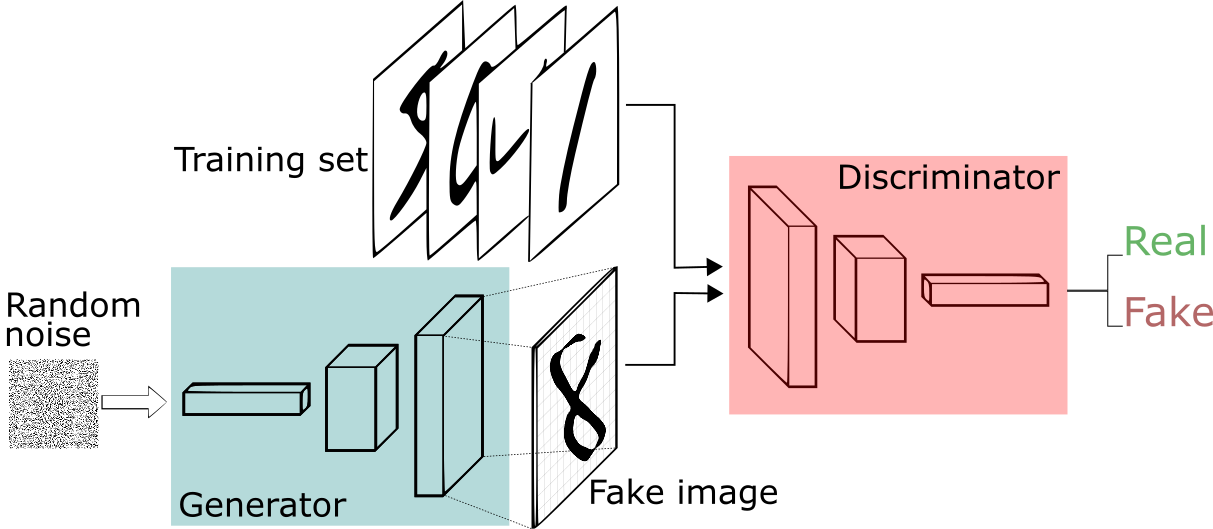
\includegraphics[width=\linewidth]{media/gan.png}
	\caption{Gan Architecture.  \textbf{https://medium.freecodecamp.org/an-intuitive-introduction-to-generative-adversarial-networks-gans-7a2264a81394}}
	\label{fig:gan}
\end{figure}

As an implementation detail, on the generator side, minimizing $-log~D(G(z))$ (or maximizing $log~D(G(z))$) is better than minimizing $log~D(1-G(z))$ since it's gradients are better for initial samples generated by $G$.

So for the discriminator, we want to maximize:

\begin{center}
	$\mathbb{E}_{x \sim P_r}~log~D(x) + \mathbb{E}_{z \sim P_z} log D(1-G(z))$
\end{center}

and for the generator, we want to maximize:

\begin{center}
	$\mathbb{E}_{z \sim P_z}~log~D(1-G(z))$
\end{center}

Since $D$ and $G$ are neural networks, we can maximize them with using Stochastic Gradient Descent. 

\section{Wasserstein GAN}

\subsection{Overview}
As mentioned in the past section, the training for GANs is usually very slow and unstable, so the Wasserstein Adversarial Network - WGAN was introduced as an improvement in order to make training less difficult. The layout of the WGAN is different than the regular GAN. Now we only have one neural network in the model, the Generator, and a system that the author of the WGAN paper REF calls the critic. Instead of using another NN to classify the data as real or fake, WGAN uses the critic to find the distance function in between a real data probability distribution and a fake one, and then uses this function to calculate the loss, and finally update the weights to start a new iteration.

\subsection{Introduction}
When training GAN models the goal is to find a distribution $P_{\theta}$ that is the most similar to a real distribution $P_{r}$, where $\theta$ is the parameters. There are two approaches to perform this task:
1. Define a parametric family of densities $P_{\theta}$, which is as a differentiable function $P_{\theta} >= 0$ and integral ($P_{\theta}$(x) dx) = 1, where x is a real data sample. Try to directly learn $P_{theta}$ by optimizing it through maximum likelihood estimation (MLE).
2. Define a variable Z with an existent distribution $p(z)$ and pass it through the Generator, $g_{\theta}$, that will generate samples that follow the distribution $P_{theta}$. By updating $\theta$ the $P_{theta}$ can be modified to get more similar to $P_{r}$.

The first approach usually runs into problems since trying to maximize MLE:
\textbf{insert MLE equation here}

Is the same as trying to minimize KL divergence.
(maybe insert proof here or just the KL equation).

In KL divergence if Q(x) = 0, which in this case is $P_{theta}$, for a $x$ where $P_{r}(x) > 0$, the result goes to +infinity. This makes improbable for $P_{r}$ to fall within that support in low dimensional manifolds, which means that if one point of $P_{theta}$ lays outside of the support, KL will not be defined. In order to try to remediate this problem, a noise term called the Gaussian noise, with a large enough bandwidth to cover all the examples, is added to the distribution $P_{theta}$. Although by taking this maneuver, error is being added to the system resulting in poor quality images. Also, even if a density $P_{theta}$ is learned, it could be computationally expensive to sample from it REF (read-through).

The latter approach has two big advantages: it can represent distributions in a low dimension manifold, and unlike the densities, it is easier to generate samples of the distribution. This specific approach is the focus of the main reference for this survey (REF WGAN paper). To get to the goal of finding a distribution  $P_{theta}$ as close to $P_{r}$ as possible, the parameter $\theta$ needs to be optimized, in which the mapping $\theta -> P_{theta}$ should be continuous, since the objective is when a sequence of parameters converge to $\theta$, the distribution correspondent to those parameters converges to $P_{theta}$. To measure the similarity, or distance in between the distributions in order to keep fine tuning $\theta$, the paper goes on to present various metrics that are commonly used. 



\section{Graph Convolutional Networks}
\subsection{Background}
\subsection{Overview}


\section{Conclusion \& Future Work}


\section*{References}

\end{document}

